% Load the kaobook class
\documentclass[
	fontsize=10pt, % Base font size
	twoside=true, % Use different layouts for even and odd pages (in particular, if twoside=true, the margin column will be always on the outside)
	%open=any, % If twoside=true, uncomment this to force new chapters to start on any page, not only on right (odd) pages
%%	secnumdepth=1, % How deep to number headings. Defaults to 1 (sections)
]{kaobook}

\newcommand{\discipline}{Informatique -- PTSI}
\newcommand{\auteur}{I. Cotta, X. Pessoles, V. Reydellet}
\newcommand{\repRel}{../../../..}

\input{\repRel/Style/packages_v2}
\newcommand{\repStyle}{\repRel/Style}
\input{\repRel/Style/macros_SII_v2}
\input{\repRel/Style/environment_v2}
\usepackage{\repStyle/UPSTI_pedagogique}


\usepackage[english,french]{babel}
\frenchsetup{StandardItemLabels=true}


% Load packages for testing
%\usepackage{blindtext}
%\usepackage{showframe} % Uncomment to show boxes around the text area, margin, header and footer
%\usepackage{showlabels} % Uncomment to output the content of \label commands to the document where they are used

% Load the bibliography package
%\usepackage{kaobiblio}
%\addbibresource{Cy_01_ModelisationSystemes.bib} % Bibliography file

% Load mathematical packages for theorems and related environments
\usepackage{kaotheorems}

% Load the package for hyperreferences
\usepackage{kaorefs}
%\usepackage{lmodern}

\graphicspath{{images/}{./}} % Paths where images are looked for

\makeindex[columns=3, title=Alphabetical Index, intoc] % Make LaTeX produce the files required to compile the index


\begin{document}

%%----------------------------------------------------------------------------------------
%%	BOOK INFORMATION
%%----------------------------------------------------------------------------------------

\titlehead{Xavier Pessoles - Informatique en PTSI}
\title[Xavier Pessoles - Informatique en PTSI]{Xavier Pessoles - Informatique en PTSI}
\author[XP]{Xavier Pessoles}
\date{\today}


\begingroup % Local scope for the following commands
\setstretch{1} % Uncomment to modify line spacing in the ToC
%\tableofcontents % Output the table of contents
\endgroup

%%----------------------------------------------------------------------------------------
%%	MAIN BODY
%%----------------------------------------------------------------------------------------
%
\mainmatter % Denotes the start of the main document content, resets page numbering and uses arabic numbers
%\setchapterstyle{kao} % Choose the default chapter heading style
%
%\chapter{First Chapter}
%
%\blindtext
%
%\pagelayout{wide} % No margins
%\addpart{Title of the Part}
%\pagelayout{margin} % Restore margins
%
%\chapter{Second Chapter}

\setchapterstyle{kao}

\setcounter{margintocdepth}{\sectiontocdepth}
\marginlayout
\graphicspath{{\repStyle/png}}

\pagestyle{xp.scrheadings}
%\pagestyle{xp.test}


%\input{\repStyle/Cycle_01_Entete}



%%%%%
\newcommand{\repExo}{Application_01_ROV}
\newcommand{\nomExo}{Application_01_ROV}
%\newcounter{cptApplication}[chapter]
%\newcounter{cptTD}[chapter]
\AtBeginEnvironment{corrige}{\small}

\livrettrue % Livrettrue :  eleve sans les corrections
\livrettrue
\colletrue
%%%%%


% ========= TD ========= 
\renewcommand{\repExo}{\repRel/Informatique/Exercices/S1_03_UtilisationModules/}
\renewcommand{\nomExo}{02_MarcheAutoEvitante}
\graphicspath{{\repStyle/png}{\repExo\nomExo/images}}


\section*{Exercice indépendant}
On souhaite analyser l'évolution de la température au cours
d'une période donnée à l'aide d'une moyenne glissante.

Voici les températures relevées : \lstinline{temperatures = [18, 20, 19, 22, 24, 23, 21, 25, 26, 24]}.


On souhaite calculer une moyenne glissante sur une fenêtre de 3 jours.


Une moyenne glissante consiste à calculer la moyenne d'un ensemble de valeurs consécutives, puis à décaler la fenêtre d'un élément pour effectuer le calcul suivant.

Par exemple, pour une fenêtre de taille 3 :
\begin{itemize}
    \item moyenne des jours 1 à 3 : 
    \(
    \frac{18+20+19}{3}=19
    \);
    \item moyenne des jours 2 à 4 :
    \(
    \frac{20+19+22}{3}=20{,}33
    \).
\end{itemize}

\subsubsection*{Travail demandé}

Écrire une fonction Python appelée \texttt{moyenne\_glissante()} qui prend deux paramètres :
\begin{itemize}
    \item \texttt{data} : une liste de valeurs numériques ;
    \item \texttt{window} : la taille de la fenêtre de calcul.
\end{itemize}

\subsubsection*{Résultat attendu}

Pour le code suivant :

\begin{lstlisting}[language=Python]
temperatures = [18, 20, 19, 22, 24, 23, 21, 25, 26, 24]
resultat = moyenne_glissante(temperatures, 3)
print(resultat)
\end{lstlisting}

On doit obtenir :

\begin{lstlisting}
[19.0, 20.33, 21.67, 23.0, 22.67, 23.0, 24.0, 25.0]
\end{lstlisting}

%\section{Contraintes}
%
%\begin{itemize}
%    \item Ne pas utiliser les bibliothèques NumPy ou Pandas.
%    \item Utiliser uniquement les fonctionnalités natives de Python.
%    \item Utiliser une boucle \texttt{for}.
%    \item Utiliser le slicing pour extraire les fenêtres :
%    \texttt{data[i:i+window]}.
%\end{itemize}
%
%\section{Bonus : pour aller plus loin}
%
%\begin{enumerate}
%    \item Ajouter une gestion des erreurs lorsque la taille de
%    la fenêtre est nulle ou supérieure à la taille de la liste.
%
%    \item Tester la fonction avec différentes tailles de fenêtre
%    (2, 3 et 5).
%
%    \item Optimiser le calcul en évitant de recalculer la somme
%    complète à chaque itération : ajouter la nouvelle valeur
%    et retirer l'ancienne.
%\end{enumerate}
%
%\end{document}


\proffalse
%\setchapterimage{fig_00.jpg}
\chapter*{TP 5 \\ 
Tracé de l'abaque de temps de réponse à 5 \% -- \ifprof Corrigé \else Sujet \fi}
\addcontentsline{toc}{section}{TP 5 : 
Tracé de l'abaque de temps de réponse à 5 \% -- \ifprof Corrigé \else Sujet \fi}

\iflivret \stepcounter{cptApplication} \else
\ifprof  \stepcounter{cptApplication} \else \fi
\fi

\setcounter{question}{0}

%\section*{}

\begin{obj}
L'objectif de ces travaux est de construire le programme permettant de tracer l'abaque du temps de réponse réduit utilisé en asservissement pour connaître le temps de réponse à 5\% des systèmes d'ordre 2. 
\end{obj}

\subsection*{Mise en situation}
\ifprof
\else

\marginnote{
On note : 
\begin{itemize}
\item $K$ : le gain statique;
\item $\xi$ : le coefficient d'amortissement;
\item $e(t)$ et $s(t)$ : l'entrée et la sortie du système. 
\end{itemize}
}
L'équation différentielle d'un système du second ordre peut se mettre sous la forme :

$$
s(t)
+\dfrac{2\xi}{\omega_0}\cdot \dfrac{\text{d}s(t)}{\text{d}t}
+\dfrac{1}{\omega_0^2}\cdot \dfrac{\text{d}^2s(t)}{\text{d}t^2}
= K\cdot e(t)
$$



On suppose que toutes les conditions initiales sont nulles. Pour une entrée unitaire de type échelon unitaire $e(t)=u(t)$, $K=1$ et $t\geq0$ on montre que : 
\begin{itemize}
\item si $\xi <1$, le régime est pseudo périodique et :
$$
s(t)=1-\dfrac{e^{-\xi\omega_0 t}}{\sqrt{1-\xi^2}}\sin\left(  \omega_0 t\sqrt{1-\xi^2}+\arcsin \sqrt{1-\xi^2} \right)
$$
\item si $\xi=1$, le régime est critique et : 
$$
s(t)=1-\left(1+\omega_0 t \right)e^{-\omega_0 t} 
$$
\item si $\xi>1$, le régime est apériodique et : 
$$
s(t)=1
+\dfrac{e^{- \omega_0 t\left( \xi + \sqrt{\xi^2-1}\right)}}{2\left(\xi\sqrt{\xi^2-1}+\xi^2-1 \right)}
-\dfrac{e^{- \omega_0 t \left( \xi - \sqrt{\xi^2-1}\right)}}{2\left(\xi\sqrt{\xi^2-1}-\xi^2+1 \right)}
$$
\end{itemize} 


\textbf{Dans l'ensemble de ce sujet, on considèrera que $s$ est une fonction du temps réduit $t\cdot\omega_0$ que l'on notera $t\omega_0$ ou \lstinline{tom0}. On notera indifféremment le coefficient d'amortissement $z$ ou $\xi$.}



\textbf{Pour répondre aux questions on utilisera la fichier \lstinline{TP_05.py} donné sur le site de la classe.}
\fi 



\subsection*{Tracé de la réponse indicielle}
\ifprof
\else
On dispose des fonctions Python \textbf{\lstinline{f_pseudo}} et \textbf{\lstinline{f_aperiodique}} permettant d'évaluer la fonction pour $s$ pour un couple $(t\omega_0,\xi)$.
\fi



\marginnote{\textbf{Test :} 
Vérifier que \lstinline{f_critique(1)} $\simeq 0,26$.}
\begin{question}
Implémenter en Python la fonction \lstinline{f_critique} permettant de calculer 
$s(t\omega_0)$ dans le cas où $\xi=1$. %Compléter la fonction \lstinline{f_critique(tom0)}.
%On respectera impérativement la syntaxe Python. Les spécifications de la fonction seront les suivantes : 
\end{question}
\ifprof
\else
%\begin{lstlisting}
%def f_critique(tom0):
%    """
%    Fonction permettant de calculer s(tom0) dans le cas ou z>1. 
%    Entrées :
%        * tom0, flt : le temps réduit - sans unité
%    Sortie : 
%        * res, flt : s(tom0) - ici, sans unité.
%    """
%\end{lstlisting}
\fi
\ifprof
\begin{lstlisting}
def f_critique(tom0):
    """
    Fonction permettant de calculer s(t) dans le cas ou z>1. 
    Entrées :
        * tom0 flt : le temps réduit - sans unité
    Sortie : 
        * res, flt : s(tom0) - ici, sans unité.
    """
    return 1-(1+tom0)*math.exp(-tom0) 
\end{lstlisting}
\else

\fi


\marginnote{\textbf{Test :} 
Vérifier que \lstinline{f_s(1,0.5),f_s(1,1),f_s(1,2)} renvoie approximativement \lstinline{0.34,0.26,0.17}.}
\begin{question}
Implémenter en Python la fonction \lstinline{f_s} permettant de calculer  $s(t\omega_0,\xi)$ dans le cas où $\xi\in \mathbb{R}_+^*$. %On donne ci-dessous les spécifications de la fonction.
\end{question}
%\ifprof
%\else
%\begin{lstlisting}
%def f_s(tom0,z):
%    """
%    Fonction permettant de calculer la réponse indicielle d'un système du second ordre. 
%    Entrées : 
%        * tom0, flt : temps de réponse réduit
%        * z, flt : coefficient d'amortissement
%    Sortie : 
%        * s(tom0,z), flt
%    """
%\end{lstlisting}
%\fi

\ifprof
\begin{corrige}
\begin{lstlisting}
def f_s(tom0,z) :
    """
    Fonction permettant de calculer la réponse indicielle d'un système du second ordre. 
    Entrées : 
        * tom0, flt : temps de réponse réduit
        * z, flt : coefficient d'amortissement
    Sortie : 
        * s(tom0,z), flt
    """
    if z<0 :
        return None
    elif z<1 :
        return f2_pseudo(tom0,z)
    elif z==1:
        return f2_critique(tom0)
    else : 
        return f2_aperiodique(tom0,z)
\end{lstlisting}
\end{corrige}
\else

\fi


\marginnote{\textbf{Test :} 
Vérifier que \lstinline{les_t[0],les_t[-1]} renvoie approximativement \lstinline{0,9.9999}.}
\begin{question}
Définir la variable \lstinline{les_t} qui contient la liste des temps. Cette liste contiendra 1000 valeurs de temps, répartie entre 0 et \SI{10}{s}. Il n'est pas nécessaire de créer une fonction pour cette question.
\end{question}


\begin{question}
Définir les variables \lstinline{les_s04} et \lstinline{les_s07} qui contienennt la liste des valeurs de $s(tom0,\xi)$ respectivement pour $\xi=0,4$ et $\xi=0,7$. Il n'est pas nécessaire de créer une fonction pour cette question.
\end{question}

\begin{question}
Tracer \lstinline{les_s04} et \lstinline{les_s07} en fonction de \lstinline{les_t}.
\end{question}


\begin{marginfigure}
\begin{center}
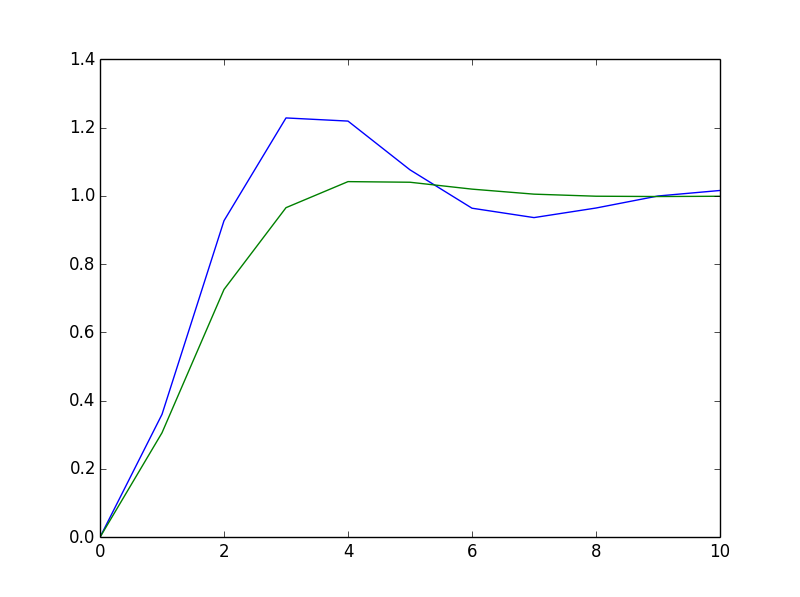
\includegraphics[width=\textwidth]{images/courbe}
\end{center}
\end{marginfigure}




\ifprof
\begin{corrige}
\begin{lstlisting}
def trace_s(z):
    x = []
    y = []
    n = 1000
    for i in range(n+1):
        t = 10*i/n
        x.append(t)
        y.append(f_s(t,z))
    plot(x,y)
\end{lstlisting}
\end{corrige}
\else
\fi

\subsection*{Tracé de l'abaque}

On note $t_r$  le temps de réponse à 5\%. L'abaque du temps de réponse permet de tracer le produit $t_r\omega_0$ en fonction du coefficient d'amortissement $\xi$.

\begin{question}
Dans les conditions de la fonction $s$ définie dans la partie précédente, quelle est la valeur finale prise par $s(t)$ ?
\end{question}
\ifprof
\begin{corrige}
La valeur finale est 1. 
\end{corrige}
\else

\fi


\begin{question}
Écrire en Python la fonction \lstinline{is_in_strip} dont les spécifications sont donner dans le fichier .py. 
\end{question}
\ifprof
\else
%\begin{lstlisting}
%def is_in_strip(x):
%    """
%    Fonction permettant de savoir si une valeur est dans la bande des + ou - 5% de la valeur finale.
%    Entrée : 
%        x, flt : réel
%    Sortie : 
%        True si la valeur est dans la bande à + ou - 5%
%        False si la valeur n'est pas dans la bande à + ou - 5%
%    """
%\end{lstlisting}
\fi

\ifprof
\begin{corrige}
\begin{lstlisting}
def is_in_strip(x):
    """
    Fonction permettant de savoir si une valeur est dans la bande des + ou - 5% de la valeur finale.
    Entrée : 
        x, flt : réel
    Sortie : 
        True si la valeur est dans la bande à + ou - 5%
        False si la valeur n'est pas dans la bande à + ou - 5%
    """
    if x>.95 and x<1.05:
        return True
    else:
        return False
\end{lstlisting}
\end{corrige}
\else



\fi

\ifprof
\else
%\vspace{1cm}

On donne la fonction \lstinline{calcul_tom0(z,tom0=500)}  permettant de connaître le temps de réponse réduit à partir duquel la réponse indicielle d'un système est dans la bande à plus ou moins 5\% pour un coefficient d'amortissement particulier.

%\begin{lstlisting}
%def calcul_tom0(z,tom0=500):
%    """
%    Recherche du temps de réponse à 5%
%    Entrées : 
%       * z, flt : coefficient d'amortissement
%       * tom0 (flt, optionnel) : si non précisé, on calcule le temps de réponse en partant de tom0 = 500
%    Sortie : 
%       * tom0 (flt) : temps de réponse à 5%
%    """
%    pas_tom0=0.05
%    x = f_s(tom0,z) 
%    if z<0.7:
%        # Dans cas, s'assurer que le tom0 initial est suffisamment grand
%        while is_in_strip(x) :
%            tom0  = tom0 - pas_tom0
%            x = f_s(tom0,z)
%        tom0=tom0+pas_tom0
%    else :
%        # Dans cas, s'assurer que le tom0 initial est suffisamment petit
%        while not is_in_strip(x) :
%            tom0  = tom0 + pas_tom0 
%            x = f_s(tom0,z)
%        tom0=tom0-pas_tom0
%    return tom0
%\end{lstlisting}


\fi


\begin{question}Expliquer le mode de recherche du temps de réponse à 5\% dans le cas où $z<0,7$ puis dans le cas où $z\geq 0,7$. Pourquoi distingue-t-on ces 2 cas ? On pourra s'aider de l'abaque donné page \pageref{ref_aba}.
\end{question}

\ifprof
\else
\begin{rem}
On pourra remarquer que dans un cas, la recherche se fait << en avançant >> et dans le second cas << en reculant >>. 
\end{rem}




\fi

\ifprof
\begin{corrige}
Pour déterminer le temps de réponse à 5\%, on cherche le dernier temps pour lequel, le signal est dans la bande à plus ou moins 5\%. En régime permanent, le signal est dans la bande. En << remontant le temps >> la première valeur hors de la bande correspond donc au temps de réponse recherché. 

Lorsque $\xi<0,7$, le système est oscillant, et le temps de réponse est mesuré lorsque les oscillations deviennent <<petites>>. Il est donc préférable de partir de la fin.

Lorsque $\xi>0,7$, on sait que dès lors que le signal entre dans la bande, il n'en sortira plus. Il est donc plus rapide de commencer par le début. 

\end{corrige}
\else
\fi

\ifprof
\else

La fontion \lstinline{make_xy()} permet de créer les listes \lstinline{xx} et \lstinline{yy} permettant de tracer l'abaque du temps de réponse réduit en fonction du coefficient d'amortissement. 

%\begin{lstlisting}
%xx,yy = [],[]
%n = 1000
%z = 0.01
%tom0 = 500
%pasz = 0.01
%while z<=100:
%    print(z)
%    if z<0.7:
%        tom0=calcul_tom0(z,tom0)
%    else :
%        tom0=calcul_tom0(z,0)
%  
%    if z<0.1:
%        pasz = 0.001
%    elif z<1:
%        pasz = 0.01
%    elif z<10:
%        pasz = 0.1
%    else :
%        pasz = 1
%    
%    xx.append(z)
%    yy.append(tom0)
%    z=z+pasz
%\end{lstlisting}

\fi


 
\begin{question}
\begin{enumerate}
\item Donner l'intervalle de variation de \lstinline{z} pour le tracé demandé.
\item Donner le pas de \lstinline{z} sur chacun des intervalles.
\item Pourquoi ne pas conserver le même pas sur chacun de ces intervalles ?
\item En vous aidant du tracé de l'abaque, expliquer pourquoi \lstinline{tom0} est calculé différemment suivant la valeur de \lstinline{z} ? Expliquer le choix des arguments de la fonction \lstinline{calcul_tom0} dans chacun des cas. 
\end{enumerate}
\end{question}
\ifprof
\begin{corrige}
\begin{enumerate}
\item $z$ variera de 0,01 à 100.
\item On a : 
\begin{itemize}
\item si $0,01<z<0,1$ : $pasz = 0,001$;
\item si $0,1<z<1$ : $pasz = 0,01$;
\item si $1<z<10$ : $pasz = 0,1$;
\item si $10<z<100$ : $pasz = 1$.
\end{itemize}
\item La courbe est tracée en diagramme log-log. On adopte donc un pas différent par décade. 
\item Lorsque $\xi<0.7$, $tom0$ décroit lorsque $z$ croît. Pour trouver plus rapidement $tom0$ on peut donc utiliser la valeur prise précédemment (dans ce cas, la recherche de tom0 dans la fonction \lstinline{calcul_tom0} se fait à rebours). A l'inverse, lorsque $\xi>0.7$, $tom0$ croit lorsque $z$ croît. On choisit dans ce cas, de partir à chaque fois de 0 (en modifiant le code, il serait possible de partir du $tom0$ calculé précédemment, mais il faudrait réfléchir à la gestion de la bascule de $\xi<0,7$ à $\xi>0,7$).
\end{enumerate}
\end{corrige}
\else
\fi
%
%\subparagraph{}
%\textit{On souhaite stocker les données des listes \lstinline{xx} et \lstinline{yy} dans un fichier texte encodé en ASCII. Chacun des nombres doit être stocké sur 17 caractères. Indiquer la taille du fichier ainsi créé.}
%\ifprof
%\begin{corrige}
%90 valeurs sont calculées pour chaque intervalles de $z$. $xx$ et $yy$ ont donc une taille de 360 éléments. 
%En prenant en compte les 34 caractères, l'espace et le retour à la ligne (2 caractères), une ligne a donc une taille de 37 octets. Le fichier sera donc d'approximativement de 13 320 octets.
%\end{corrige}
%\else
%
%\begin{tabular}{|p{.95\textwidth}|}
%\hline
%$$\quad$$
%\vspace{2cm}
%$$\quad$$ \\
%\hline
%\end{tabular}
%
%\fi
\ifprof
\else

%
%\begin{lstlisting}
%import matplotlib.pyplot as plt
%import numpy as np
%
%plt.plot(xx,yy,label="Temps de réponse réduit $tr \\omega_0$")
%plt.xlabel("Coefficient d'amortissement $\\xi$")
%plt.ylabel("Temps de réponse réduit $tr \\omega_0$")
%plt.title("Temps de réponse réduit d'un système du 2nd ordre")
%plt.legend()
%plt.loglog()
%plt.grid(which="major",axis="x",linewidth=1.5, linestyle='-')
%plt.grid(which="major",axis="y",linewidth=1.5, linestyle='-')
%plt.grid(which="minor",axis="x",linewidth=0.75, linestyle='-', color='0.75')
%plt.grid(which="minor",axis="y",linewidth=0.75, linestyle='-', color='0.75')
%\end{lstlisting}

\begin{question}
Tracer l'abaque en utilisant la fonction \lstinline{plot_abaque(xx,yy)}.
\end{question}
\begin{figure}[!ht]
\centering
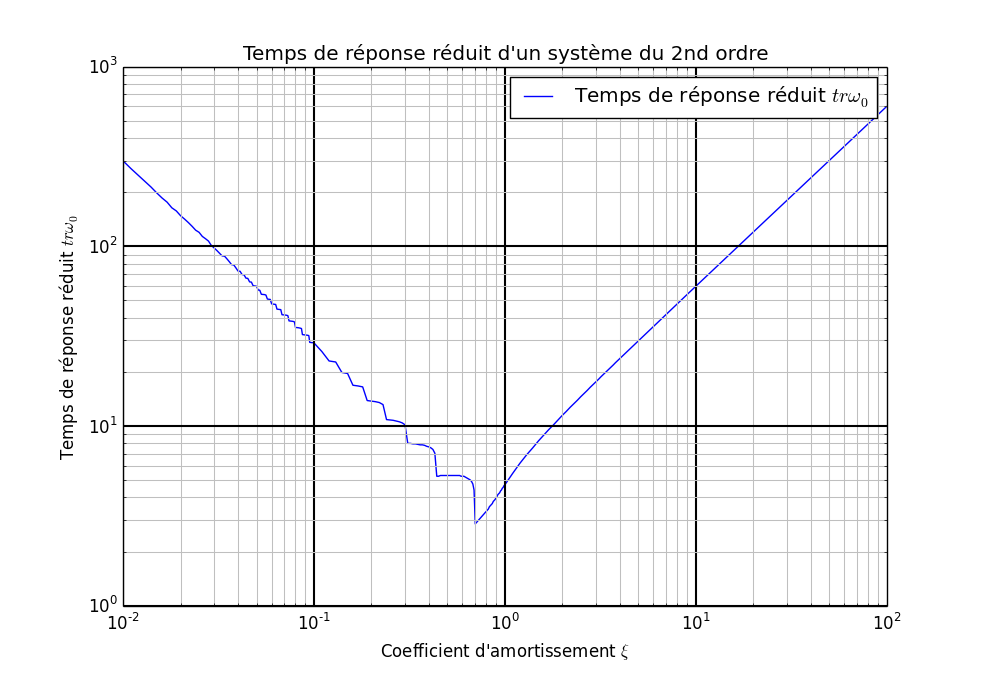
\includegraphics[width=.7\linewidth]{images/figure_1}

\caption{Abaque du temps de réponse réduit pour un système du second ordre \label{ref_aba}}
\end{figure}
\fi
\end{document}
 
\iflivret \else \proftrue
%\setchapterimage{fig_00.jpg}
\chapter*{TP 5 \\ 
Tracé de l'abaque de temps de réponse à 5 \% -- \ifprof Corrigé \else Sujet \fi}
\addcontentsline{toc}{section}{TP 5 : 
Tracé de l'abaque de temps de réponse à 5 \% -- \ifprof Corrigé \else Sujet \fi}

\iflivret \stepcounter{cptApplication} \else
\ifprof  \stepcounter{cptApplication} \else \fi
\fi

\setcounter{question}{0}

%\section*{}

\begin{obj}
L'objectif de ces travaux est de construire le programme permettant de tracer l'abaque du temps de réponse réduit utilisé en asservissement pour connaître le temps de réponse à 5\% des systèmes d'ordre 2. 
\end{obj}

\subsection*{Mise en situation}
\ifprof
\else

\marginnote{
On note : 
\begin{itemize}
\item $K$ : le gain statique;
\item $\xi$ : le coefficient d'amortissement;
\item $e(t)$ et $s(t)$ : l'entrée et la sortie du système. 
\end{itemize}
}
L'équation différentielle d'un système du second ordre peut se mettre sous la forme :

$$
s(t)
+\dfrac{2\xi}{\omega_0}\cdot \dfrac{\text{d}s(t)}{\text{d}t}
+\dfrac{1}{\omega_0^2}\cdot \dfrac{\text{d}^2s(t)}{\text{d}t^2}
= K\cdot e(t)
$$



On suppose que toutes les conditions initiales sont nulles. Pour une entrée unitaire de type échelon unitaire $e(t)=u(t)$, $K=1$ et $t\geq0$ on montre que : 
\begin{itemize}
\item si $\xi <1$, le régime est pseudo périodique et :
$$
s(t)=1-\dfrac{e^{-\xi\omega_0 t}}{\sqrt{1-\xi^2}}\sin\left(  \omega_0 t\sqrt{1-\xi^2}+\arcsin \sqrt{1-\xi^2} \right)
$$
\item si $\xi=1$, le régime est critique et : 
$$
s(t)=1-\left(1+\omega_0 t \right)e^{-\omega_0 t} 
$$
\item si $\xi>1$, le régime est apériodique et : 
$$
s(t)=1
+\dfrac{e^{- \omega_0 t\left( \xi + \sqrt{\xi^2-1}\right)}}{2\left(\xi\sqrt{\xi^2-1}+\xi^2-1 \right)}
-\dfrac{e^{- \omega_0 t \left( \xi - \sqrt{\xi^2-1}\right)}}{2\left(\xi\sqrt{\xi^2-1}-\xi^2+1 \right)}
$$
\end{itemize} 


\textbf{Dans l'ensemble de ce sujet, on considèrera que $s$ est une fonction du temps réduit $t\cdot\omega_0$ que l'on notera $t\omega_0$ ou \lstinline{tom0}. On notera indifféremment le coefficient d'amortissement $z$ ou $\xi$.}



\textbf{Pour répondre aux questions on utilisera la fichier \lstinline{TP_05.py} donné sur le site de la classe.}
\fi 



\subsection*{Tracé de la réponse indicielle}
\ifprof
\else
On dispose des fonctions Python \textbf{\lstinline{f_pseudo}} et \textbf{\lstinline{f_aperiodique}} permettant d'évaluer la fonction pour $s$ pour un couple $(t\omega_0,\xi)$.
\fi



\marginnote{\textbf{Test :} 
Vérifier que \lstinline{f_critique(1)} $\simeq 0,26$.}
\begin{question}
Implémenter en Python la fonction \lstinline{f_critique} permettant de calculer 
$s(t\omega_0)$ dans le cas où $\xi=1$. %Compléter la fonction \lstinline{f_critique(tom0)}.
%On respectera impérativement la syntaxe Python. Les spécifications de la fonction seront les suivantes : 
\end{question}
\ifprof
\else
%\begin{lstlisting}
%def f_critique(tom0):
%    """
%    Fonction permettant de calculer s(tom0) dans le cas ou z>1. 
%    Entrées :
%        * tom0, flt : le temps réduit - sans unité
%    Sortie : 
%        * res, flt : s(tom0) - ici, sans unité.
%    """
%\end{lstlisting}
\fi
\ifprof
\begin{lstlisting}
def f_critique(tom0):
    """
    Fonction permettant de calculer s(t) dans le cas ou z>1. 
    Entrées :
        * tom0 flt : le temps réduit - sans unité
    Sortie : 
        * res, flt : s(tom0) - ici, sans unité.
    """
    return 1-(1+tom0)*math.exp(-tom0) 
\end{lstlisting}
\else

\fi


\marginnote{\textbf{Test :} 
Vérifier que \lstinline{f_s(1,0.5),f_s(1,1),f_s(1,2)} renvoie approximativement \lstinline{0.34,0.26,0.17}.}
\begin{question}
Implémenter en Python la fonction \lstinline{f_s} permettant de calculer  $s(t\omega_0,\xi)$ dans le cas où $\xi\in \mathbb{R}_+^*$. %On donne ci-dessous les spécifications de la fonction.
\end{question}
%\ifprof
%\else
%\begin{lstlisting}
%def f_s(tom0,z):
%    """
%    Fonction permettant de calculer la réponse indicielle d'un système du second ordre. 
%    Entrées : 
%        * tom0, flt : temps de réponse réduit
%        * z, flt : coefficient d'amortissement
%    Sortie : 
%        * s(tom0,z), flt
%    """
%\end{lstlisting}
%\fi

\ifprof
\begin{corrige}
\begin{lstlisting}
def f_s(tom0,z) :
    """
    Fonction permettant de calculer la réponse indicielle d'un système du second ordre. 
    Entrées : 
        * tom0, flt : temps de réponse réduit
        * z, flt : coefficient d'amortissement
    Sortie : 
        * s(tom0,z), flt
    """
    if z<0 :
        return None
    elif z<1 :
        return f2_pseudo(tom0,z)
    elif z==1:
        return f2_critique(tom0)
    else : 
        return f2_aperiodique(tom0,z)
\end{lstlisting}
\end{corrige}
\else

\fi


\marginnote{\textbf{Test :} 
Vérifier que \lstinline{les_t[0],les_t[-1]} renvoie approximativement \lstinline{0,9.9999}.}
\begin{question}
Définir la variable \lstinline{les_t} qui contient la liste des temps. Cette liste contiendra 1000 valeurs de temps, répartie entre 0 et \SI{10}{s}. Il n'est pas nécessaire de créer une fonction pour cette question.
\end{question}


\begin{question}
Définir les variables \lstinline{les_s04} et \lstinline{les_s07} qui contienennt la liste des valeurs de $s(tom0,\xi)$ respectivement pour $\xi=0,4$ et $\xi=0,7$. Il n'est pas nécessaire de créer une fonction pour cette question.
\end{question}

\begin{question}
Tracer \lstinline{les_s04} et \lstinline{les_s07} en fonction de \lstinline{les_t}.
\end{question}


\begin{marginfigure}
\begin{center}
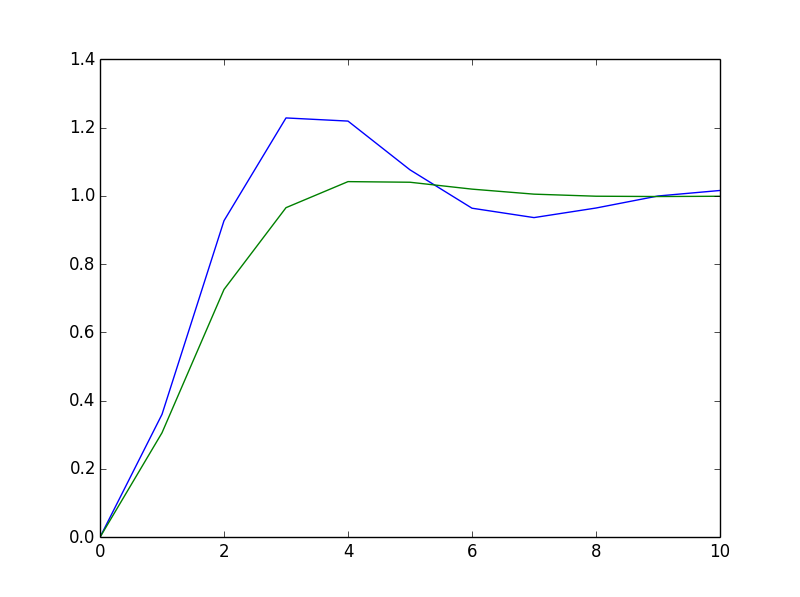
\includegraphics[width=\textwidth]{images/courbe}
\end{center}
\end{marginfigure}




\ifprof
\begin{corrige}
\begin{lstlisting}
def trace_s(z):
    x = []
    y = []
    n = 1000
    for i in range(n+1):
        t = 10*i/n
        x.append(t)
        y.append(f_s(t,z))
    plot(x,y)
\end{lstlisting}
\end{corrige}
\else
\fi

\subsection*{Tracé de l'abaque}

On note $t_r$  le temps de réponse à 5\%. L'abaque du temps de réponse permet de tracer le produit $t_r\omega_0$ en fonction du coefficient d'amortissement $\xi$.

\begin{question}
Dans les conditions de la fonction $s$ définie dans la partie précédente, quelle est la valeur finale prise par $s(t)$ ?
\end{question}
\ifprof
\begin{corrige}
La valeur finale est 1. 
\end{corrige}
\else

\fi


\begin{question}
Écrire en Python la fonction \lstinline{is_in_strip} dont les spécifications sont donner dans le fichier .py. 
\end{question}
\ifprof
\else
%\begin{lstlisting}
%def is_in_strip(x):
%    """
%    Fonction permettant de savoir si une valeur est dans la bande des + ou - 5% de la valeur finale.
%    Entrée : 
%        x, flt : réel
%    Sortie : 
%        True si la valeur est dans la bande à + ou - 5%
%        False si la valeur n'est pas dans la bande à + ou - 5%
%    """
%\end{lstlisting}
\fi

\ifprof
\begin{corrige}
\begin{lstlisting}
def is_in_strip(x):
    """
    Fonction permettant de savoir si une valeur est dans la bande des + ou - 5% de la valeur finale.
    Entrée : 
        x, flt : réel
    Sortie : 
        True si la valeur est dans la bande à + ou - 5%
        False si la valeur n'est pas dans la bande à + ou - 5%
    """
    if x>.95 and x<1.05:
        return True
    else:
        return False
\end{lstlisting}
\end{corrige}
\else



\fi

\ifprof
\else
%\vspace{1cm}

On donne la fonction \lstinline{calcul_tom0(z,tom0=500)}  permettant de connaître le temps de réponse réduit à partir duquel la réponse indicielle d'un système est dans la bande à plus ou moins 5\% pour un coefficient d'amortissement particulier.

%\begin{lstlisting}
%def calcul_tom0(z,tom0=500):
%    """
%    Recherche du temps de réponse à 5%
%    Entrées : 
%       * z, flt : coefficient d'amortissement
%       * tom0 (flt, optionnel) : si non précisé, on calcule le temps de réponse en partant de tom0 = 500
%    Sortie : 
%       * tom0 (flt) : temps de réponse à 5%
%    """
%    pas_tom0=0.05
%    x = f_s(tom0,z) 
%    if z<0.7:
%        # Dans cas, s'assurer que le tom0 initial est suffisamment grand
%        while is_in_strip(x) :
%            tom0  = tom0 - pas_tom0
%            x = f_s(tom0,z)
%        tom0=tom0+pas_tom0
%    else :
%        # Dans cas, s'assurer que le tom0 initial est suffisamment petit
%        while not is_in_strip(x) :
%            tom0  = tom0 + pas_tom0 
%            x = f_s(tom0,z)
%        tom0=tom0-pas_tom0
%    return tom0
%\end{lstlisting}


\fi


\begin{question}Expliquer le mode de recherche du temps de réponse à 5\% dans le cas où $z<0,7$ puis dans le cas où $z\geq 0,7$. Pourquoi distingue-t-on ces 2 cas ? On pourra s'aider de l'abaque donné page \pageref{ref_aba}.
\end{question}

\ifprof
\else
\begin{rem}
On pourra remarquer que dans un cas, la recherche se fait << en avançant >> et dans le second cas << en reculant >>. 
\end{rem}




\fi

\ifprof
\begin{corrige}
Pour déterminer le temps de réponse à 5\%, on cherche le dernier temps pour lequel, le signal est dans la bande à plus ou moins 5\%. En régime permanent, le signal est dans la bande. En << remontant le temps >> la première valeur hors de la bande correspond donc au temps de réponse recherché. 

Lorsque $\xi<0,7$, le système est oscillant, et le temps de réponse est mesuré lorsque les oscillations deviennent <<petites>>. Il est donc préférable de partir de la fin.

Lorsque $\xi>0,7$, on sait que dès lors que le signal entre dans la bande, il n'en sortira plus. Il est donc plus rapide de commencer par le début. 

\end{corrige}
\else
\fi

\ifprof
\else

La fontion \lstinline{make_xy()} permet de créer les listes \lstinline{xx} et \lstinline{yy} permettant de tracer l'abaque du temps de réponse réduit en fonction du coefficient d'amortissement. 

%\begin{lstlisting}
%xx,yy = [],[]
%n = 1000
%z = 0.01
%tom0 = 500
%pasz = 0.01
%while z<=100:
%    print(z)
%    if z<0.7:
%        tom0=calcul_tom0(z,tom0)
%    else :
%        tom0=calcul_tom0(z,0)
%  
%    if z<0.1:
%        pasz = 0.001
%    elif z<1:
%        pasz = 0.01
%    elif z<10:
%        pasz = 0.1
%    else :
%        pasz = 1
%    
%    xx.append(z)
%    yy.append(tom0)
%    z=z+pasz
%\end{lstlisting}

\fi


 
\begin{question}
\begin{enumerate}
\item Donner l'intervalle de variation de \lstinline{z} pour le tracé demandé.
\item Donner le pas de \lstinline{z} sur chacun des intervalles.
\item Pourquoi ne pas conserver le même pas sur chacun de ces intervalles ?
\item En vous aidant du tracé de l'abaque, expliquer pourquoi \lstinline{tom0} est calculé différemment suivant la valeur de \lstinline{z} ? Expliquer le choix des arguments de la fonction \lstinline{calcul_tom0} dans chacun des cas. 
\end{enumerate}
\end{question}
\ifprof
\begin{corrige}
\begin{enumerate}
\item $z$ variera de 0,01 à 100.
\item On a : 
\begin{itemize}
\item si $0,01<z<0,1$ : $pasz = 0,001$;
\item si $0,1<z<1$ : $pasz = 0,01$;
\item si $1<z<10$ : $pasz = 0,1$;
\item si $10<z<100$ : $pasz = 1$.
\end{itemize}
\item La courbe est tracée en diagramme log-log. On adopte donc un pas différent par décade. 
\item Lorsque $\xi<0.7$, $tom0$ décroit lorsque $z$ croît. Pour trouver plus rapidement $tom0$ on peut donc utiliser la valeur prise précédemment (dans ce cas, la recherche de tom0 dans la fonction \lstinline{calcul_tom0} se fait à rebours). A l'inverse, lorsque $\xi>0.7$, $tom0$ croit lorsque $z$ croît. On choisit dans ce cas, de partir à chaque fois de 0 (en modifiant le code, il serait possible de partir du $tom0$ calculé précédemment, mais il faudrait réfléchir à la gestion de la bascule de $\xi<0,7$ à $\xi>0,7$).
\end{enumerate}
\end{corrige}
\else
\fi
%
%\subparagraph{}
%\textit{On souhaite stocker les données des listes \lstinline{xx} et \lstinline{yy} dans un fichier texte encodé en ASCII. Chacun des nombres doit être stocké sur 17 caractères. Indiquer la taille du fichier ainsi créé.}
%\ifprof
%\begin{corrige}
%90 valeurs sont calculées pour chaque intervalles de $z$. $xx$ et $yy$ ont donc une taille de 360 éléments. 
%En prenant en compte les 34 caractères, l'espace et le retour à la ligne (2 caractères), une ligne a donc une taille de 37 octets. Le fichier sera donc d'approximativement de 13 320 octets.
%\end{corrige}
%\else
%
%\begin{tabular}{|p{.95\textwidth}|}
%\hline
%$$\quad$$
%\vspace{2cm}
%$$\quad$$ \\
%\hline
%\end{tabular}
%
%\fi
\ifprof
\else

%
%\begin{lstlisting}
%import matplotlib.pyplot as plt
%import numpy as np
%
%plt.plot(xx,yy,label="Temps de réponse réduit $tr \\omega_0$")
%plt.xlabel("Coefficient d'amortissement $\\xi$")
%plt.ylabel("Temps de réponse réduit $tr \\omega_0$")
%plt.title("Temps de réponse réduit d'un système du 2nd ordre")
%plt.legend()
%plt.loglog()
%plt.grid(which="major",axis="x",linewidth=1.5, linestyle='-')
%plt.grid(which="major",axis="y",linewidth=1.5, linestyle='-')
%plt.grid(which="minor",axis="x",linewidth=0.75, linestyle='-', color='0.75')
%plt.grid(which="minor",axis="y",linewidth=0.75, linestyle='-', color='0.75')
%\end{lstlisting}

\begin{question}
Tracer l'abaque en utilisant la fonction \lstinline{plot_abaque(xx,yy)}.
\end{question}
\begin{figure}[!ht]
\centering
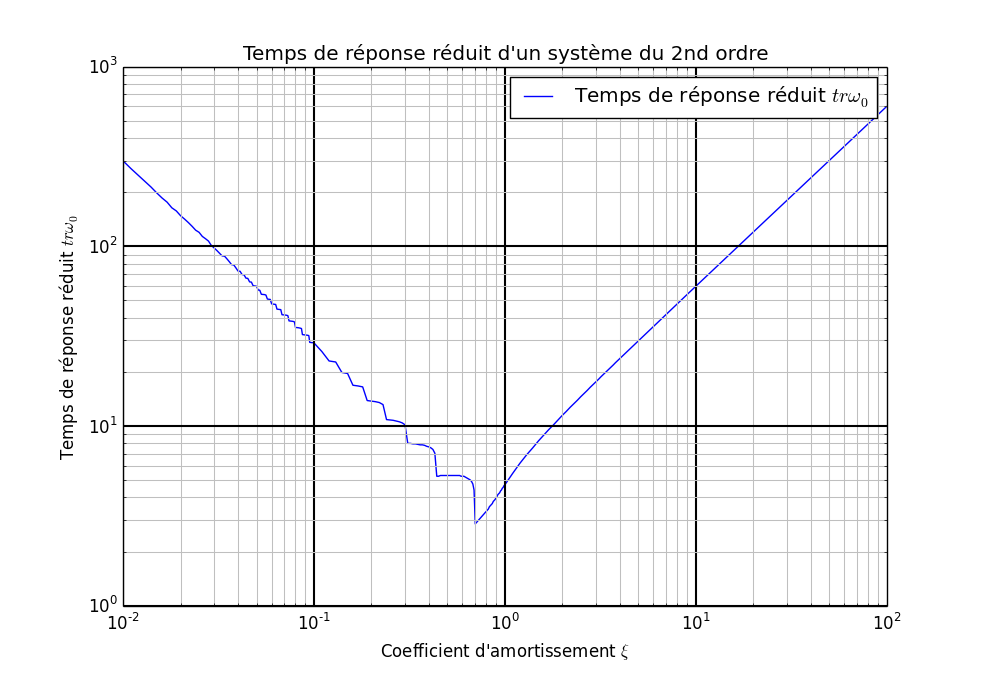
\includegraphics[width=.7\linewidth]{images/figure_1}

\caption{Abaque du temps de réponse réduit pour un système du second ordre \label{ref_aba}}
\end{figure}
\fi
\end{document}

\fi
% ===




%
%\proffalse
%\input{\repExo\nomExo/\nomExo} 
%\iflivret \else \proftrue
%\input{\repExo\nomExo/\nomExo}
%\fi
%% ==========================





\end{document}
